\section{A delivered information intervention is not necessarily an effective one}
\label{sec:native-advice}

The count/content study changes some inputs without exceeding strong rules.
Before attributing this to absent information or launching a larger search,
we test whether a particular institutional message reaches the relevant native
decision at the intended time. This is a developer intervention, not a newly
invented institution or an independent optimization history.

\paragraph{Fixed contrast and native world.}
At source\code{5925d5b}, three original four-year worlds use the same five
Qwen3-8B researchers, explicitly reused development seed61001, base30 resource
profile, M1 history, conserving equalization and unchanged T/U measurement.
The literal message recommends choosing a permitted short-duration topic; it
does not change the displayed catalog, choose a topic for a researcher or
overwrite project dates. The three conditions cut delivery, deliver at phase2
before the first direction choices, or deliver at phase235 after those choices.
The message and all three conditions are fixed before dispatch, not chosen
from favorable responses. A permission-only preparation stop precedes the
separately recorded successful launch; no scientific slot was consumed there
or replaced. All three worlds subsequently close normally.

\begin{table}[t]
\centering\small
\begin{tabular}{lrrrrr}
\toprule
Condition & Advice in inputs & Shortest choice & Mean duration & T & U\\
\midrule
Cut &0/10 &4/10 &2.6 & $-7$ & $-4$\\
Early &10/10 &4/10 &2.6 & $-7$ & $-4$\\
Late &5/10 &4/10 &2.6 & $-7$ & $-4$\\
\bottomrule
\end{tabular}
\caption{All three literal advice-timing controls. Advice presence is checked
in actual direction-request inputs, not inferred from node execution.
Duration is the selected topic's displayed catalog duration in years, averaged
over ten requests per world. Shortest is relative to that request's permitted
catalog; following the advice is not a validity requirement. The late message
is absent from first-year direction inputs, as declared. These are one-seed
developer contrasts, not independent search replications.}
\label{tab:native-advice}
\end{table}

\paragraph{Delivery established; the proposed choice effect absent here.}
All30 direction requests are uniquely joined to their original stored memories
and displayed catalog. Early and late delivery each store five addressed
instruction records; cut stores none. The exact literal text occurs in0/10,
10/10 and5/10 direction inputs, respectively. Nevertheless, every corresponding
actor/year chooses the same topic and catalog duration across all three worlds
(Table~\ref{tab:native-advice}). Each chooses a shortest displayed option on
four of ten requests, with mean selected duration2.6 years, and all yield
T=$-7$/U=$-4$. Non-shortest choices are not schema violations: the message is
advice, not a mandatory native law. We retain those choices and their losses
rather than rewriting them to satisfy the instruction.

\begin{figure}[t]
\centering
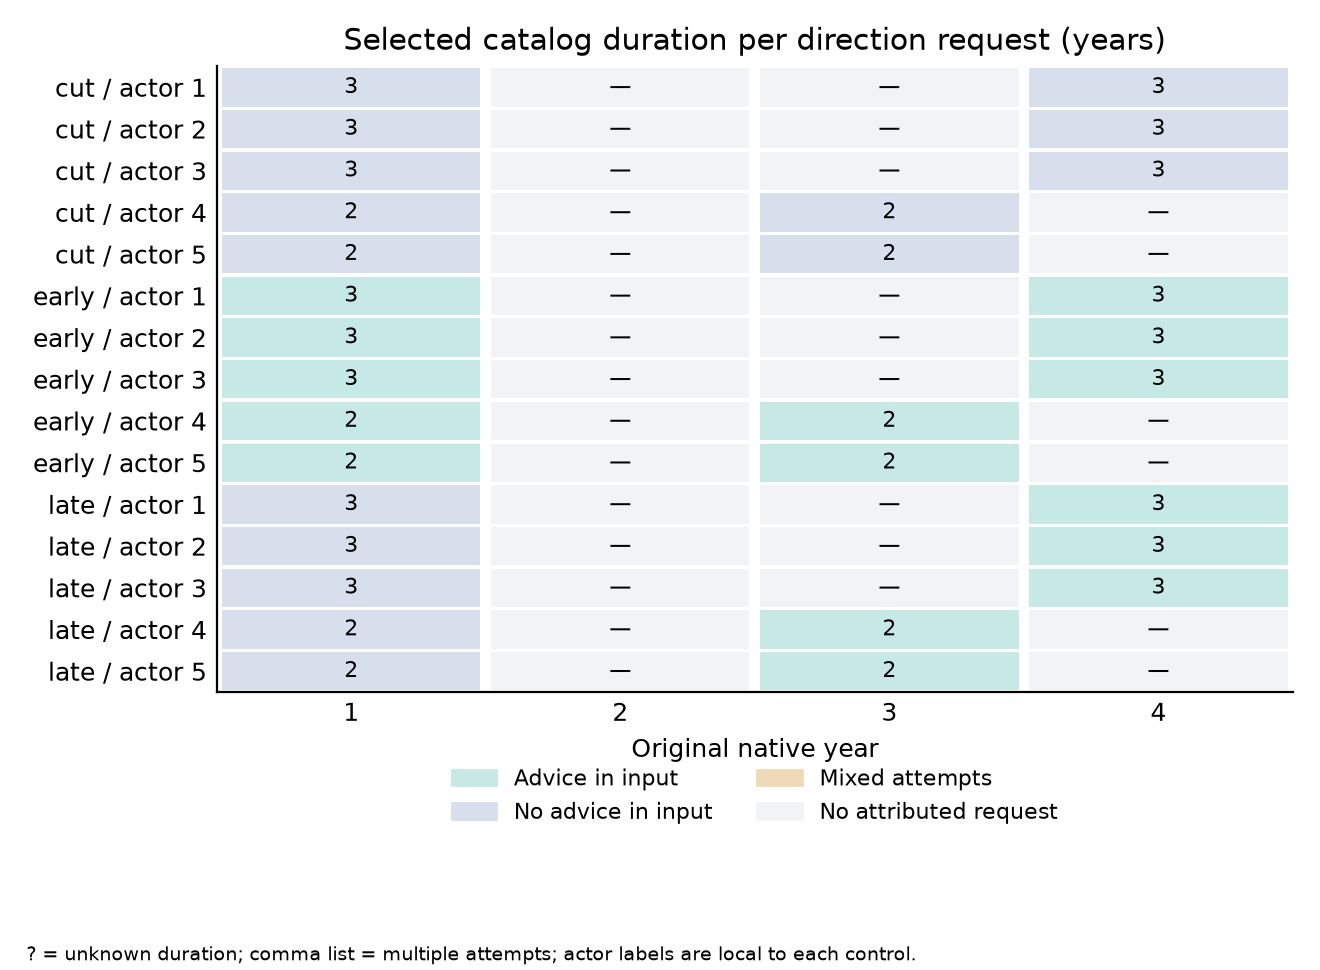
\includegraphics[width=\linewidth]{figures/native-instruction-timing-v1/choice-years.png}
\caption{Actual annual direction-input delivery and catalog-duration choices
in the three closed native worlds. The original displayed catalog and literal
received action determine each point. Delivery varies at the declared times;
the observed selected durations coincide. This supports a scoped delivery/choice
distinction, not a general inability of information institutions to affect
researchers or a causal account of why this message did not change topics.}
\label{fig:native-advice}
\end{figure}

\paragraph{Equal selected choices do not imply equivalent worlds.}
The complete ordered model-input and literal-response sequences differ among
all three worlds. Cut has129 completed scientist replies, early and late130
each. Total author resources at year4 are350,310 and350, respectively. Thus
unchanged topics, durations and T/U are weaker than behavioral equivalence or
identical resource trajectories. Resource diagnostics do not add an adoption
veto or another term to either optimization loss.

\paragraph{Audit, costs and inference boundary.}
Two original-source cold audits and two cost projections agree; the choice,
effect and complete-input exports and repeated summary/figures also agree.
Actual native execution takes about24min, followed by about1m15s of cold/report
closure. There are389 scientist replies with360734 input and38542 output
tokens;63873 cached input tokens are a subset. The unchanged content observer
uses39 separate requests. Tokenless model-load costs remain unknown; there
are no designer proposals. The result establishes that this literal message
was delivered and did not improve these particular choices or T/U at this
seed. It does not establish general instruction ineffectiveness, equal full
behavior, scientific quality, a policy ranking or a benefit of graph search.
All exact data, message identity, source and closure receipts are retained in
\path{research/data/native-instruction-timing-v1/}.
\FloatBarrier
